\chapter{Conclusiones}

La división que se hizo de los datos es estadísticamente  adecuada.

Se encontró que el AG es una buena opción para solucionar este problema de maximización.

Este trabajo apoya las necesidades de los alumnos de la Facultad.

Con el fin de encontrar más posibles aplicaciones del programa realizado en este trabajo, se buscaron diferentes páginas de horarios en distintas facultades de la UNAM y de otras universidades. No se pudieron encontrar páginas con todas las características que tienen las páginas de la Facultad. Algunas de las páginas que se encontraron son las siguientes:

\begin{itemize}
\item[-] \textit{Facultad de Filosofía y Letras UNAM:} Se encontró una estructura en las páginas web con las cuales se puede acceder a la información por carrera, pero no se puede acceder a la información de semestres anteriores y dentro de éstas páginas no se pueden encontrar el número de alumnos inscritos por cada materia, por lo que no sería posible una simulación del número de alumnos.

\url{https://servicios-galileo.filos.unam.mx/horarios/ordinarios/1354}

\url{https://servicios-galileo.filos.unam.mx/horarios/ordinarios/1355}

\url{https://servicios-galileo.filos.unam.mx/horarios/ordinarios/1359}


%\item[-] \textit{Facultad de Ingeniería UNAM:} En la siguiente página web se puede seleccionar una materia y buscar la información de ella del semestre en curso, no se puede acceder a información de semestres anteriores y no se tiene alguna estructura para buscar de manera automática los datos.
%
%\url{https://www.ssa.ingenieria.unam.mx/horarios.html}
%
%Una vez que se ingresa a la materia, se puede encontrar información del salón, horario, cupo y vacantes, se podría obtener el número de alumnos inscritos al restar el cupo del número de vacantes, pero al no tener información de semestres anteriores en todo momento, la recopilación de información tardaría años.

\item[-] \textit{FES Acatlán (Actuaría):} En la siguiente página web se pueden descargar los horarios del semestre en curso en un archivo de Excel el cual no contiene información del número de alumnos inscritos en el grupo, tampoco se puede obtener información de semestres anteriores. No se puede utilizar la aplicación \textit{SelectorGadget} para obtener la información.

\url{http://www.actuaria.acatlan.unam.mx/}

\item[-] \textit{FES Iztacala (Psicología):} Se encontró una estructura en las páginas web con las cuales se puede acceder a la información en archivos pdf de algunos semestres, dependiendo si el semestre en curso es par o impar. No se puede utilizar la aplicación \textit{SelectorGadget} para obtener la información.

%\url{https://psicologia.iztacala.unam.mx/avisos2020/horarios21_1/21-1_1-PRIMERSEMESTRE_1409.pdf}

\url{https://psicologia.iztacala.unam.mx/avisos2020/horarios21_1/21-1_3-TERCER\%20SEMESTRE.pdf}

\url{https://psicologia.iztacala.unam.mx/avisos2020/horarios21_1/21-1_5-QUINTO\%20SEMESTREv1108.pdf}

\item[-] \textit{Centro de Nanociencias y Nanotecnología (Nanotecnología):} Al igual que en el caso anterior la información de las páginas que se muestran a continuación están en archivos pdf por lo que no se puede utilizar la aplicación \textit{SelectorGadget} para obtener la información.

\url{https://nanolic.cnyn.unam.mx/sitio/wp-content/uploads/2020/09/H-1A-2021-1.pdf}

\url{https://nanolic.cnyn.unam.mx/sitio/wp-content/uploads/2020/09/H-1B-2021-1.pdf}

\url{https://nanolic.cnyn.unam.mx/sitio/wp-content/uploads/2020/09/H-3A-2021-1.pdf}

\item[-] \textit{Facultad de Química UNAM:} En la siguiente página web se pueden seleccionar todas las materias impartidas en la facultad o por carrera.

\url{http://escolares.quimica.unam.mx/Horarios/hor_def_e2.php4}

Una vez que se eligió alguna opción, se muestra un listado, en la siguiente url, con las posibles materias que se pueden elegir.

\url{http://escolares.quimica.unam.mx/Horarios/hor_def_pre_e2.php4}

Finalmente se accede a la información con la siguiente página web.

\url{http://escolares.quimica.unam.mx/Horarios/hor_tot_e2.php4}

No importa las opciones que se elijan, siempre se obtienen esas mismas urls por lo que no hay alguna estructura para poder buscar la información automáticamente.


%\item[-] \textit{ESIME Zacatenco IPN (Ingeniería en Control y Automatización):} Se encontró una estructura en las páginas web pero no se puede encontrar el número de alumnos inscritos por materia por lo que no es posible realizar una simulación del número de alumnos.
%
%\url{http://horarios.esimez.ipn.mx/horarios/VHorGpoAl.aspx?Gpo=1AM8&PaId=57}
%
%\url{http://horarios.esimez.ipn.mx/horarios/VHorGpoAl.aspx?Gpo=1AV1&PaId=57}
%
%\url{http://horarios.esimez.ipn.mx/horarios/VHorGpoAl.aspx?Gpo=5AM3&PaId=57}
%
%\url{http://horarios.esimez.ipn.mx/horarios/VHorGpoAl.aspx?Gpo=5AV3&PaId=57}


\item[-] \textit{ITAM:} En este caso se debe de seleccionar una materia y luego se despliega la información, sin importar la selección de la materia, las url son las mismas por lo que no se tiene una estructura en las páginas web.

\url{http://escolar1.rhon.itam.mx/licenciaturas/horarios/seleccion_03.asp}

\url{http://escolar1.rhon.itam.mx/licenciaturas/horarios/pormateria_03.asp}

\begin{figure}[H]
\centering
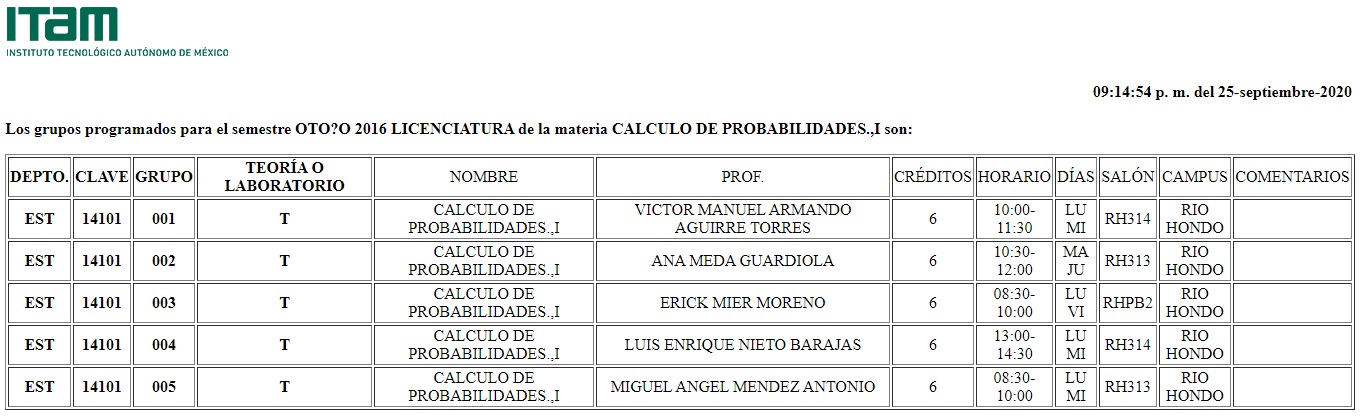
\includegraphics[scale = 0.45]{ITAM_Proba_I} %width=\textwidth
%\url{http://www.fciencias.unam.mx/docencia/horarios/20181/2017/625} %%URL de la imagen
\caption{\textit{ITAM Probabilidad I}}
\end{figure}


\item[-] \textit{Universidad La Salle:} Se encontró que las páginas tienen una cierta estructura y también se tiene la información del número de alumnos inscritos por materia pero los archivos son pdf por lo que no se puede utilizar la aplicación \textit{SelectorGadget} para obtener la información.

\url{https://cienciasquimicas.lasalle.mx/wp-content/uploads/2020/08/QFB-291.pdf}

\url{https://cienciasquimicas.lasalle.mx/wp-content/uploads/2020/08/QFB-391.pdf}

\url{https://cienciasquimicas.lasalle.mx/wp-content/uploads/2020/08/QFB-991.pdf}


\item[-] \textit{Universidad Panamericana:} No se encontraron horarios de materias, sólo de exámenes y de entrenamientos.

\url{https://www.up.edu.mx/sites/default/files/fechas_de_examenes_humanidades_1202.pdf}

\url{https://www.up.edu.mx/en/media/22960}

\end{itemize}

Sólo se encontró la misma estructura en las otras carreras de la Facultad, por lo que se puede ajustar el programa realizado en este trabajo para ellas. Algunas consideraciones que se deberían de tomar en cuenta son por ejemplo que las materias impartidas en los laboratorios duran más de una hora, no todas las materias se imparten todos los días, existen varias materias que no duran horas enteras. A continuación se presentan algunos ejemplos:

\begin{itemize}
\item[-] \textit{Biología:}

\url{http://www.fciencias.unam.mx/docencia/horarios/20172/181/1601}

\item[-] \textit{Ciencias de la Tierra:}

\url{http://www.fciencias.unam.mx/docencia/horarios/20182/1439/1318}

\item[-] \textit{Física:}

\url{http://www.fciencias.unam.mx/docencia/horarios/20191/1081/830}

\item[-] \textit{Física Biomédica:}

\url{http://www.fciencias.unam.mx/docencia/horarios/20192/2016/1735}

\item[-] \textit{Manejo Sustentable de Zonas Costeras:}

\url{http://www.fciencias.unam.mx/docencia/horarios/20181/1262/386}

\end{itemize}

